\documentclass[a4paper,11pt]{scrartcl}

\usepackage{fullpage}
\usepackage[utf8]{inputenc}
\usepackage[english]{babel}
\usepackage{amsmath}
\usepackage{amssymb}
\usepackage{commath}
\usepackage{hyperref}
\usepackage{graphicx}

\newcommand{\R}{\mathbb{R}}

\begin{document}

\section{Smoothed Prolongation for $H^1$}
We want to construct an improved prolongation operator
$P: \R^{ncv} \rightarrow \R^{nv}: u_c \mapsto u_f$ for $H^1$ algebraic multigrid.

\subsection{Notation}
\begin{itemize}
  \item ne \dots number of fine edges
  \item nv \dots number of fine vertices
  \item ncv \dots number of coarse vertices
\end{itemize}

\subsection{Idea}
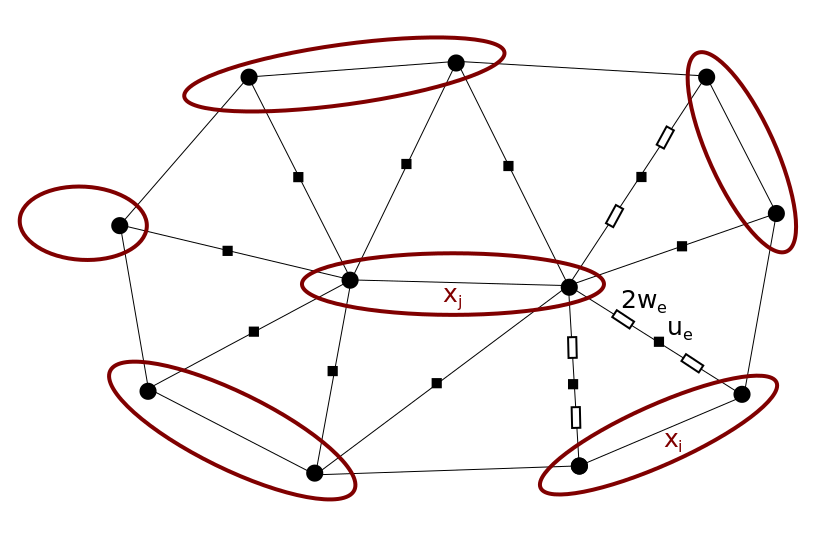
\includegraphics[width=0.6\linewidth]{pictures/h1_smoothed_diagram.png}

Given is $u_c$ on the coarse grid. $u_f$ on the fine grid is determined as following on each patch
around a coarse vertex:
\begin{enumerate}
  \item Introduce extra potentials in the midpoints of edges fine edges and assign the average
        of the corresponding coarse edge potentials.
        Compute for each fine edge between coarse vertices $x_i$ and $x_j$:
        \[ u_{E_{ij}} = \frac{u_{c_i} + u_{c_j}}{2} \]
  \item For each fine vertex corresponding to coarse vertex $x_j$
    \[ u_j = \text{Solution of Graph-Laplace with } u_E \text{ as boundary conditions} \]

\end{enumerate}

\subsection{Implementation}
We calculate the smoothed prolongation matrix in two steps:
\begin{enumerate}
  \item averaging the coarse vertices for $u_e$ of the fine edges gives rise to matrix
    $A \in \R^{ne \times ncv}$

    \begin{equation*}
      A =
      \begin{pmatrix}
        1/2 & 1/2 &  0 \\
        1/2 & 1/2 &  0 \\
        1/2 & 1/2 &  0 \\
        1/2 &  0  & 1/2 \\
        1/2 &  0  & 1/2
      \end{pmatrix}
    \end{equation*}


  \item solving the graph laplace $L$ with $u_e$ as Dirichlet BC gives rise to matrix
    $B \in \R^{nv \times ne}$
    from the equation:
    \begin{equation*}
      \begin{pmatrix}
        I & 0 \\
        L_{ve} & L_{vv}
      \end{pmatrix}
      \begin{pmatrix}
        u_e \\
        u_v
      \end{pmatrix}
      = 0
    \end{equation*}
    \[ u_v = - L^{-1}_{vv} L_{ve} u_e = B u_e \]
    \[ B = - L^{-1}_{vv} L_{ve} \]

    \[ (\Delta_{\gamma} \phi)(v) = \sum_{w: d(w,v)=1} \gamma_{wv}[\phi(v) - \phi(w)] \]
    thus:
    \begin{equation*}
      L_{uv} =
      \begin{cases}
        \sum_{w: d(u,w)=1} \gamma_{uw} & \text{if } u=v,\\
        -\gamma_{uv}& \text{otherwise}
      \end{cases}
    \end{equation*}

\end{enumerate}

\[ P_{patch} = B A \in \R^{nv \times ncv} \]

\subsection{References:}
\begin{itemize}
  \item \url{https://en.wikipedia.org/wiki/Discrete_Laplace_operator}\newline
  \item \url{https://en.wikipedia.org/wiki/Laplacian_matrix}
\end{itemize}

\section{Semi-Smoothed Prolongation for $H^1$}
\[ D = diag(A) \]
cf. $P_{semi} = (I - D^{-1} A) P_{triv}$ if $A$ is the graph-laplace matrix

\[ {(D^{-1} A)}_{i} = \frac{1}{a_{ii}} \del{a_{i1} \dots a_{in}} \]
\[ I - \frac{1}{2} {(D^{-1} A)}_{i} = \frac{1}{a_{ii}} \del{a_{i1} \dots \frac{a_{ii}}{2} \dots a_{in}} \]
\[ a_{ii} = \sum_{j} w_{e_{ij}} \quad a_{ij} = - w_{e_{ij}} \]

\[ u_i = \sum_{j} \frac{w_{e_{ij}}}{\sum_{j} w_{e_{ij}}}\frac{u_{c_i} + u_{c_j} }{2}
       = \frac{1}{2} u_{c_i} + \sum_{j} \frac{w_{e_{ij}}}{\sum_{j} w_{e_{ij}}} \frac{u_{c_j}}{2} \]

\end{document}
